\begin{figure}[h] 
\centering 
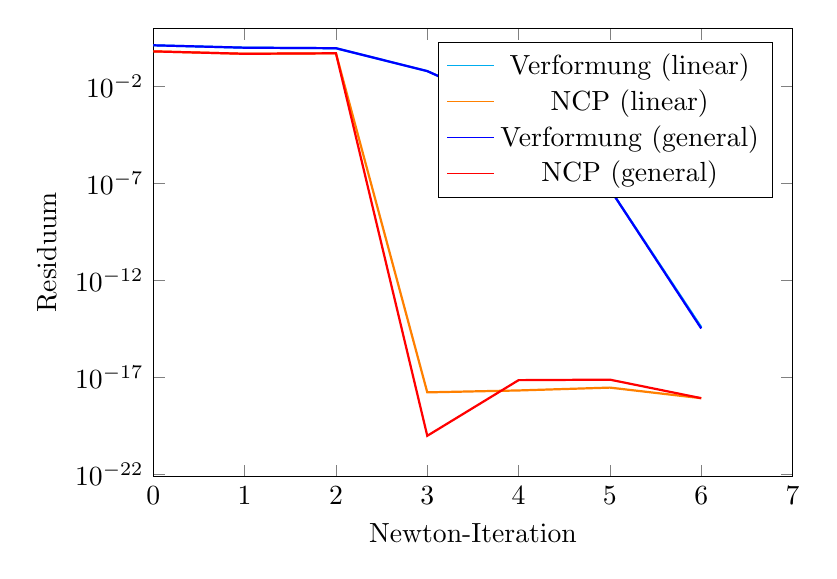
\begin{tikzpicture}[every plot/.append style={thick}] 
\begin{axis}[ 
label style={font=\normalsize}, 
xlabel={Newton-Iteration}, 
ylabel={Residuum}, 
xmin=0, xmax=7, 
ymode=log, 
ymin=0, ymax=10, 
width=0.8\textwidth, 
height=0.6\textwidth, 
legend pos=north east, 
legend style={cells={align=left}}, 
grid style=dashed, 
] 
\addplot[ 
color=cyan, 
] 
coordinates { 
(0, 1.32e+00)(1, 9.94e-01)(2, 9.33e-01)(3, 6.17e-02)(4, 4.88e-04)(5, 5.20e-08)(6, 3.93e-15)}; 
\addlegendentry{Verformung (linear)} 
\addplot[ 
color=orange, 
] 
coordinates { 
(0, 6.42e-01)(1, 4.82e-01)(2, 5.12e-01)(3, 1.73e-18)(4, 2.17e-18)(5, 3.04e-18)(6, 8.67e-19)}; 
\addlegendentry{NCP (linear)} 
\addplot[ 
color=blue, 
] 
coordinates { 
(0, 1.32e+00)(1, 9.94e-01)(2, 9.33e-01)(3, 6.17e-02)(4, 4.88e-04)(5, 5.20e-08)(6, 3.39e-15)}; 
\addlegendentry{Verformung (general)} 
\addplot[ 
color=red, 
] 
coordinates { 
(0, 6.42e-01)(1, 4.82e-01)(2, 5.12e-01)(3, 1.00e-20)(4, 7.37e-18)(5, 7.81e-18)(6, 8.67e-19)}; 
\addlegendentry{NCP (general)} 
\end{axis} 
\end{tikzpicture} 
\caption{Residuen des Stoffgesetzes 'St.Venant' mit Hinderniss 'Spitze' und 162 Freiheitsgraden für die Verschiebung.} 
\label{fiq:St.Venant_Spitze_level2} 
\end{figure} 
